\documentclass[11pt,a4paper]{article}
\usepackage[french]{babel}
\usepackage[T1]{fontenc}
\usepackage{lmodern}
\usepackage[margin=2cm]{geometry}
\usepackage{graphicx}
\usepackage{booktabs}
\usepackage{amsmath}
\usepackage{caption}
\usepackage{hyperref}
\usepackage{enumitem}
\usepackage{float}

\hypersetup{hidelinks}
\captionsetup{font=small, labelfont=bf}
\setlist{nosep, leftmargin=*}
\setlength{\parskip}{0.4em}

\title{Projet ALG 2026 : FM-index coloré\\
\large Comparaison d'un FM-index généralisé et de N FM-index avec filtres de Bloom}
\author{Matys Dulong et Corentin Perrot -- M2 Bioinformatique Rennes}
\date{Octobre 2026}

\begin{document}
\maketitle

\section{Choix d'implémentation}

Le code est écrit en Python 3.12 ; son utilisation est décrite dans le
README. Les génomes sont lus avec pyfastx : chaque séquence d'un fichier
FASTA est un contig, gardé séparé des autres.

\paragraph{FM-index (\texttt{fm\_index.py}).} Le suffix array est calculé avec
pydivsufsort puis jeté : seuls la BWT (une chaîne), la table Count
(\texttt{first\_occurrence}, une entrée par lettre de \texttt{\$ACGT}) et la
table Rank (\texttt{occ}) sont conservés. \texttt{occ} est complète : pour
chaque lettre, une liste de $n+1$ entiers donnant le nombre d'occurrences de
la lettre dans \texttt{bwt[0:i]}. Le rang est donc lu en $O(1)$ et la
recherche arrière d'une requête $q$ coûte $O(|q|)$, au prix d'une table de
$5(n+1)$ entiers.

\paragraph{Approche 1 : FM-index généralisé (\texttt{generalized\_index.py}).}
Le texte indexé est la concaténation de tous les contigs de tous les génomes,
chacun suivi de \texttt{\$}. Comme les requêtes ne contiennent pas de
\texttt{\$}, une requête ne peut pas être trouvée à cheval sur deux contigs ou
deux génomes. Le color array est rempli à partir du suffix array : la case $i$
reçoit le numéro du génome (ordre du FOF) où commence le suffixe de la ligne
$i$. Une requête est cherchée une seule fois : on lit les couleurs de
l'intervalle \texttt{[top, bottom]} renvoyé par la recherche arrière.

\paragraph{Approche 2 : N FM-index et N filtres de Bloom (\texttt{bf\_index.py}).}
Pour chaque génome, on construit un FM-index de ses contigs séparés par
\texttt{\$} et un filtre de Bloom de $m$ bits (bitarray) avec $h$ fonctions
de hachage (mmh3 avec les graines $0$ à $h-1$), rempli avec tous les
$k$-mers de chaque contig (aucun $k$-mer à cheval sur deux contigs). Pour une
requête, on teste son premier $k$-mer dans chaque filtre et on n'interroge
que les FM-index dont le filtre répond oui. Un filtre de Bloom n'a pas de
faux négatif, et ses faux positifs sont corrigés par le FM-index : le
résultat est donc exact. Une requête plus courte que $k$ n'a pas de premier
$k$-mer : tous les FM-index sont alors interrogés.

\paragraph{Programmes et validation.} \texttt{index\_colored\_fm\_index.py}
et \texttt{query.py} suivent l'interface du sujet ; les paramètres des
filtres sont ajoutés en options (\texttt{-k}, \texttt{-{}-bloom\_size},
\texttt{-{}-num\_hashes}, défauts 21, $2^{24}$ et 3). L'index est sérialisé
avec pickle et les temps mesurés avec \texttt{time.perf\_counter} ;
\texttt{TIME\_BUILD} ne compte pas la lecture des FASTA. 23 tests pytest
valident chaque structure. En particulier, \texttt{test\_consistency.py}
vérifie que les deux approches et une recherche naïve (\texttt{q in contig})
donnent le même résultat sur 350 requêtes et des génomes aléatoires qui se
recouvrent, puis sur 200 requêtes réelles E.~coli, et que les deux programmes
produisent des fichiers de résultats identiques.

Nous n'avons pas implémenté d'optimisation (couleurs sur $\lceil\log_2
N\rceil$ bits, échantillonnage de \texttt{occ}) : la section~\ref{sec:conclusion}
explique, à partir de nos mesures, laquelle serait la plus utile.

\section{Protocole expérimental}

\paragraph{Données.} Les 4 collections fournies sur Moodle, de 49 génomes
chacune : des génomes d'E.~coli tronqués à leurs 10\,kb ou 100\,kb
(premiers contigs, 1 à 33 contigs par génome, 94 à 98\,kb pour la version
100\,kb) et des génomes aléatoires de 10\,kb ou 100\,kb (un contig). Pour
chaque collection, 1960 requêtes de 100\,pb et 196 requêtes de 1000\,pb.
Les requêtes aléatoires sont toutes présentes dans exactement un génome ;
celles d'E.~coli sont présentes en moyenne dans 2,4 génomes (100\,pb, au plus
16) et 1,0 à 1,2 génome (1000\,pb), car les souches partagent des séquences,
et quelques-unes (jusqu'à 5\,\%) ne sont présentes dans aucun génome.

\paragraph{Expérience 1 (comparaison des approches).}
\texttt{benchmark.py} lance les deux programmes, comme un utilisateur, sur les
$N = 5, 10, 20, 35, 49$ premiers génomes de chaque collection, avec les
paramètres par défaut ($k = 21$, $h = 3$, $m = 2^{24}$). On relève les quatre
temps affichés par les programmes, la taille du fichier sérialisé, et la
taille de l'index relu en mémoire vive (\texttt{pympler.asizeof}, une seule
fois par configuration). Les temps sont la moyenne de 3 répétitions.

\paragraph{Expérience 2 (paramètres des filtres).} Sur les 49 génomes
E.~coli de 100\,kb et les 1960 requêtes de 100\,pb, on fait varier un
paramètre à la fois autour de $k = 21$, $m = 2^{20}$, $h = 3$. Le taux de
faux positifs est, parmi les couples (requête, génome) où le premier
$k$-mer est absent du génome (vérifié sur les contigs), la part où le filtre
répond oui. On mesure aussi la part de FM-index interrogés \og pour rien\fg{}
(le filtre répond oui mais la requête est absente du génome, faux positifs
compris).

\paragraph{Machine.} Linux, 8 c\oe urs, 7,6\,Go de RAM, Python 3.12.16. La
machine était chargée (swap utilisé) : d'une passe complète à l'autre, les
temps absolus ont varié jusqu'à un facteur 2,7 (temps de requête), mais
l'ordre entre les deux approches est resté le même. Nous interprétons donc surtout des rapports
entre approches. Toutes les commandes de reproduction sont dans le README.

\section{Résultats}

\subsection*{Résultat 1 : la construction et la mémoire}

\begin{figure}[H]
\centering
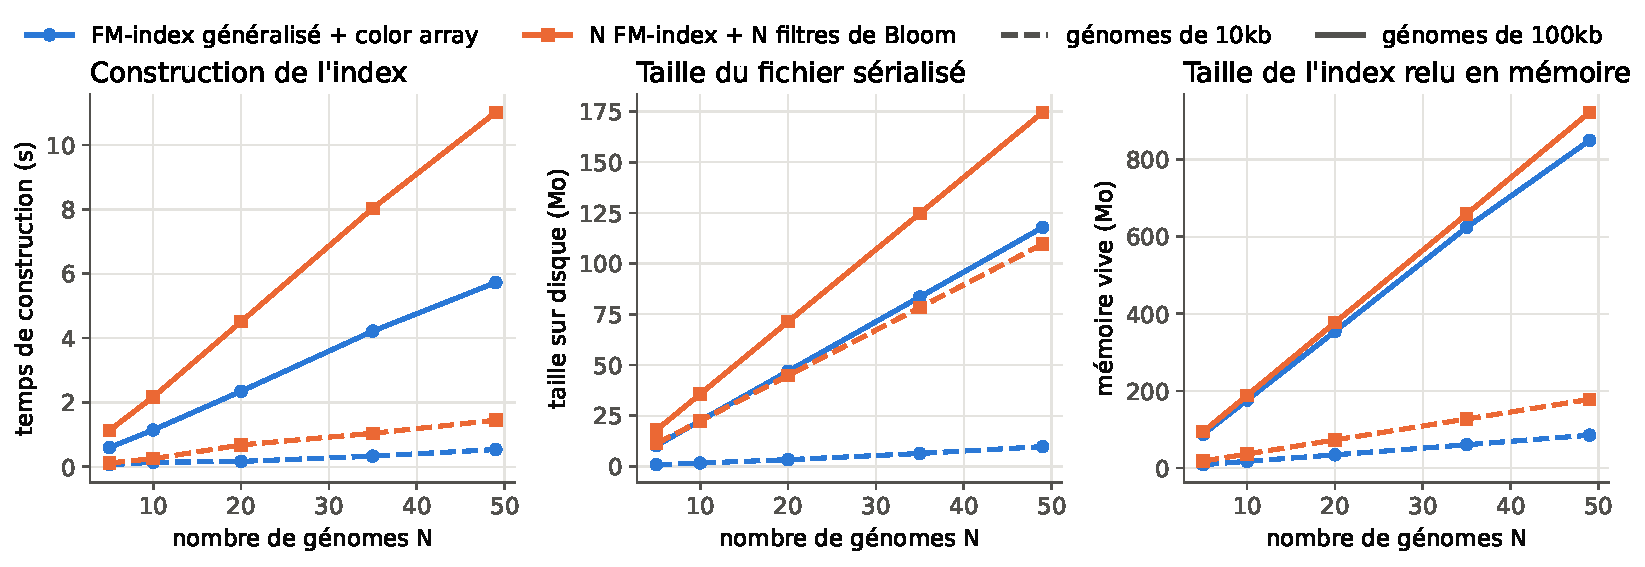
\includegraphics[width=\textwidth]{figures/fig1_construction_taille.pdf}
\caption{\textbf{Temps de construction, taille sur disque et taille en mémoire
vive des deux index selon le nombre de génomes N.} Collections E.~coli de
10\,kb (tirets) et 100\,kb (traits pleins) ; $k = 21$, $h = 3$, $m = 2^{24}$
pour \texttt{bf}. Temps : moyenne de 3 répétitions.}
\label{fig:construction}
\end{figure}

\textbf{Interprétation.} Les trois mesures croissent linéairement avec la
taille totale des génomes. \texttt{bf} se construit environ 2 fois moins vite
(11,0\,s contre 5,7\,s pour 49 génomes de 100\,kb) : en plus des N FM-index,
il faut hacher $h$ fois chacun des 4,8 millions de $k$-mers en Python
(l'expérience 2 montre que chaque fonction de hachage en plus coûte environ
0,9\,s). Sur disque, \texttt{bf} est plus gros avec le $m$ par défaut :
chaque filtre fait 2\,Mo quelle que soit la taille du génome, ce qui
représente 103\,Mo des 110\,Mo de l'index pour des génomes de 10\,kb.

Surtout, \textbf{la taille sur disque sous-estime fortement la mémoire vive}
: 118\,Mo sur disque contre 850\,Mo en RAM pour \texttt{generalized} (facteur
7 à 11 selon les configurations), 175\,Mo contre 923\,Mo pour \texttt{bf}. En mesurant
chaque attribut séparément, la table \texttt{occ} représente à elle seule
807\,Mo (95\,\%), contre 38\,Mo pour le color array et 5\,Mo pour la BWT.
En effet, pickle écrit chaque entier sur 2 à 5 octets, alors qu'une fois
relu, chaque entier de \texttt{occ} est un objet Python d'environ 28 octets,
plus 8 octets de pointeur dans la liste ($5 \times 4{,}8\cdot 10^6 \times
36 \approx 860$\,Mo). Le facteur est plus faible pour \texttt{bf} (5,3 à
100\,kb, 1,6 à 10\,kb) car ses filtres (bitarray) ont la même taille sur
disque et en mémoire. En RAM, les deux approches sont donc proches (9\,\%
d'écart à 49 génomes de 100\,kb), car elles stockent le même nombre total
d'entrées dans \texttt{occ}. Le temps de désérialisation suit le nombre
d'objets Python à recréer plutôt que la taille du fichier
(annexe~\ref{annexe}, figure~\ref{fig:deserialisation}).

\subsection*{Résultat 2 : les requêtes, \texttt{generalized} fait moins de travail}

\begin{figure}[H]
\centering
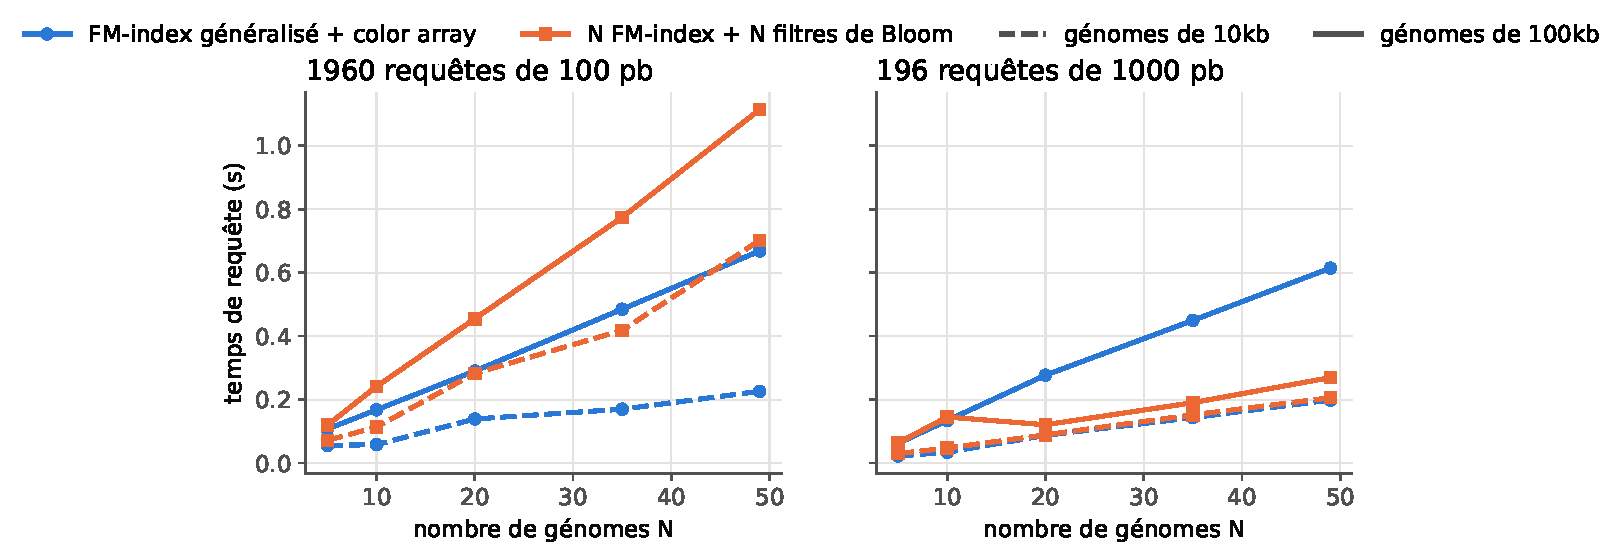
\includegraphics[width=0.92\textwidth]{figures/fig2_requetes.pdf}
\caption{\textbf{Temps total des requêtes selon le nombre de génomes N, pour
des requêtes de 100\,pb (gauche) et de 1000\,pb (droite).} Collections
E.~coli ; même légende que la figure~\ref{fig:construction}. Le temps est
mesuré par \texttt{query.py}, juste après la relecture de l'index.}
\label{fig:requetes}
\end{figure}

\textbf{Interprétation.} Pour 1960 requêtes de 100\,pb, \texttt{generalized}
est plus rapide (0,67\,s contre 1,11\,s pour 49 génomes de 100\,kb). C'est ce
qu'on attend : \texttt{generalized} fait une seule recherche arrière par
requête, alors que \texttt{bf} teste d'abord le premier $k$-mer dans les
49 filtres (4\,\textmu s par filtre, soit environ 0,4\,s pour les 1960
requêtes), puis fait une recherche dans chaque génome dont le filtre répond
oui. Comme les souches d'E.~coli partagent beaucoup de $k$-mers, c'est le cas
de 4 génomes en moyenne (jusqu'à 16), et \texttt{bf} fait au total 2,9 fois
plus d'étapes de recherche arrière (291 contre 100 par requête), pour un coût
par étape identique dans les deux index (0,6 à 0,8\,\textmu s).

Pour 196 requêtes de 1000\,pb, \texttt{bf} est au contraire mesuré plus
rapide par \texttt{query.py} (0,27\,s contre 0,61\,s). Ce résultat ne
s'explique pas par les structures : \texttt{bf} fait là encore plus de
travail (4 recherches et 1533 étapes par requête en moyenne, contre 993
étapes pour \texttt{generalized}). Mesurées dans un script séparé, sur les
mêmes index, ces requêtes prennent d'ailleurs 0,12 à 0,13\,s avec
\texttt{generalized} contre 0,19 à 0,25\,s avec \texttt{bf}. L'écart mesuré
par \texttt{query.py} dépend donc des conditions d'exécution juste après la
relecture d'un gros index, et nous ne le retenons pas comme un avantage de
\texttt{bf}.

\subsection*{Résultat 3 : la taille des filtres suit la théorie, et $m = 2^{20}$ suffit}

\begin{figure}[H]
\centering
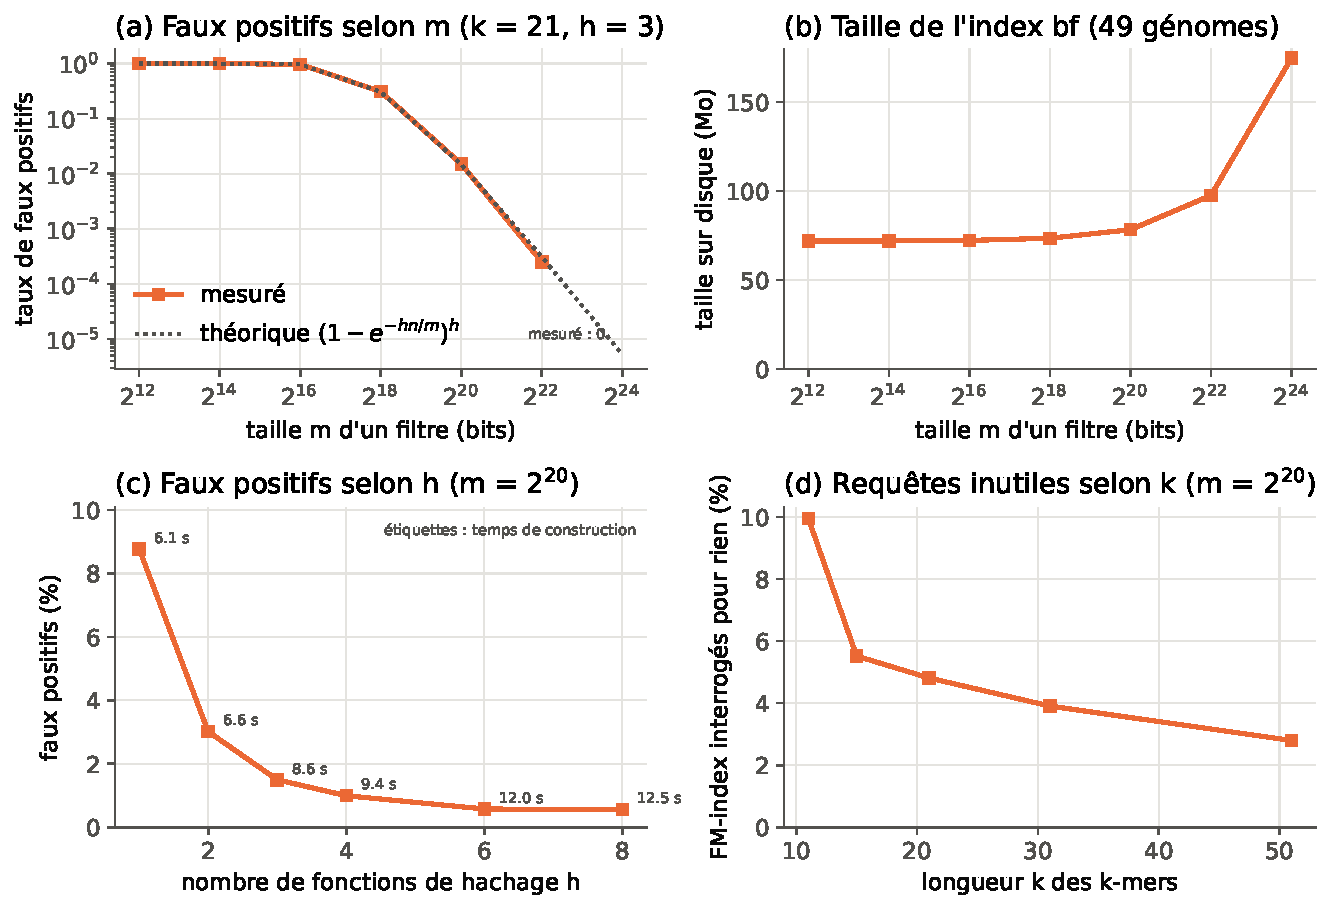
\includegraphics[width=0.78\textwidth]{figures/fig4_parametres_bloom.pdf}
\caption{\textbf{Effet des paramètres des filtres de Bloom sur l'index
\texttt{bf}.} 49 génomes E.~coli de 100\,kb, 1960 requêtes de 100\,pb ; un
seul paramètre varie, autour de $k = 21$, $m = 2^{20}$, $h = 3$.
(a)~Taux de faux positifs selon la taille $m$ d'un filtre (échelles log),
comparé à la formule théorique avec $n \approx 98\,000$ $k$-mers par génome.
(b)~Taille du fichier sérialisé selon $m$. (c)~Taux de faux positifs selon le
nombre $h$ de fonctions de hachage ; les étiquettes donnent le temps de
construction. (d)~Part des couples (requête, génome) où un FM-index est
interrogé pour rien, selon $k$.}
\label{fig:bloom}
\end{figure}

\textbf{Interprétation (a, b).} Le taux de faux positifs mesuré suit la
formule $(1 - e^{-hn/m})^h$ : 31\,\% contre 30,6\,\% attendus pour
$m = 2^{18}$, 1,50\,\% contre 1,46\,\% pour $m = 2^{20}$. Les $h$ fonctions
de notre filtre (mmh3 avec des graines différentes) se comportent donc comme
des fonctions de hachage indépendantes. Jusqu'à $2^{16}$ bits, les filtres
sont saturés (presque tous les bits à 1) : 47 à 49 FM-index sont interrogés
par requête au lieu de 4 à 5,
et les requêtes sont 2 à 3 fois plus lentes (1,6 à 2,0\,s contre 0,66 à
0,70\,s à partir de $2^{20}$). Au-dessus de $2^{20}$, les faux positifs ne coûtent
presque plus rien, mais la taille explose : les 49 FM-index seuls font
72\,Mo, et les filtres ajoutent $49 \times m/8$ octets, soit 6\,Mo pour
$2^{20}$ mais 103\,Mo pour $2^{24}$. \textbf{$m = 2^{20}$ (environ 10 bits
par $k$-mer) est un bon choix pour des génomes de 100\,kb} : 1,5\,\% de faux
positifs et un index de 78\,Mo, plus petit que celui de \texttt{generalized}
(118\,Mo). Cette différence vient surtout de pickle : dans un génome de
100\,kb, les valeurs de \texttt{occ} restent sous 65\,536 et sont écrites sur
3 octets au plus, alors qu'elles dépassent cette valeur dans l'index
généralisé et prennent alors 5 octets. Notre valeur par
défaut ($2^{24}$) est donc surdimensionnée pour ces données.

\textbf{Interprétation (c, d).} Augmenter $h$ fait baisser les faux
positifs (8,8\,\% pour $h = 1$, 1,5\,\% pour $h = 3$, 0,55\,\% pour
$h = 8$), mais chaque $k$-mer est haché $h$ fois et la construction passe de
6,1 à 12,5\,s. La théorie donne un optimum $h = (m/n)\ln 2 \approx 7$ pour
$m = 2^{20}$, mais le gain au-delà de $h = 3$ ou 4 est faible par rapport au
coût. $k$ change peu le taux de faux positifs (1,2 à 1,5\,\%, car le
nombre de $k$-mers par génome varie peu), mais un premier $k$-mer plus long
est plus spécifique : la part de FM-index interrogés pour rien passe de
10\,\% ($k = 11$) à 2,8\,\% ($k = 51$). $k$ ne doit cependant pas dépasser
la longueur des requêtes : pour une requête plus courte que $k$, le filtre
n'est pas utilisé.

\subsection*{Résultat 4 : le type de données change peu les performances}

\begin{table}[H]
\centering
\small
\caption{\textbf{Récapitulatif pour N = 49 génomes, par collection.} Temps
en secondes (moyenne de 3 répétitions), tailles en Mo. Désérialisation :
moyenne des deux fichiers de requêtes. Paramètres par défaut pour
\texttt{bf} ($m = 2^{24}$).}
\label{tab:recap}
\begin{tabular}{lllrrrrrrr}
\toprule
& & & \multicolumn{2}{c}{indexation} & \multicolumn{2}{c}{taille (Mo)} & & \multicolumn{2}{c}{requêtes} \\
\cmidrule(lr){4-5} \cmidrule(lr){6-7} \cmidrule(lr){9-10}
données & génomes & méthode & constr. & sérial. & disque & RAM & désérial. & 100\,pb & 1000\,pb \\
\midrule
coli & 10\,kb & generalized & 0{,}54 & 0{,}12 & 9{,}8 & 85 & 0{,}12 & 0{,}23 & 0{,}20 \\
coli & 10\,kb & bf & 1{,}45 & 0{,}39 & 109{,}7 & 178 & 0{,}33 & 0{,}70 & 0{,}21 \\
coli & 100\,kb & generalized & 5{,}73 & 1{,}01 & 117{,}9 & 850 & 1{,}17 & 0{,}67 & 0{,}61 \\
coli & 100\,kb & bf & 11{,}02 & 1{,}44 & 174{,}6 & 923 & 1{,}65 & 1{,}11 & 0{,}27 \\
\midrule
random & 10\,kb & generalized & 0{,}56 & 0{,}11 & 10{,}2 & 88 & 0{,}12 & 0{,}21 & 0{,}20 \\
random & 10\,kb & bf & 1{,}57 & 0{,}39 & 109{,}9 & 182 & 0{,}37 & 0{,}38 & 0{,}17 \\
random & 100\,kb & generalized & 5{,}97 & 1{,}05 & 120{,}5 & 892 & 1{,}18 & 0{,}62 & 0{,}64 \\
random & 100\,kb & bf & 11{,}78 & 1{,}14 & 176{,}1 & 936 & 1{,}75 & 0{,}82 & 0{,}19 \\
\bottomrule
\end{tabular}
\end{table}

\textbf{Interprétation.} À taille égale, les génomes E.~coli et aléatoires
donnent les mêmes temps de construction et les mêmes tailles : un FM-index
contient autant d'entrées quel que soit le contenu du texte. Les conclusions
des résultats 1 et 2 valent donc pour les deux types de données. La seule
différence concerne les requêtes de \texttt{bf} : elles ont tendance à être
plus lentes sur E.~coli (1,11\,s contre 0,82\,s pour 100\,pb à 100\,kb). Les
souches partagent beaucoup de $k$-mers : le premier $k$-mer d'une requête se
trouve souvent dans plusieurs génomes (4 en moyenne), si bien que plus de
FM-index sont interrogés, alors que chaque requête aléatoire n'est présente
que dans un seul génome.
Des génomes aléatoires, qui ne partagent presque aucun $k$-mer, sont donc le
cas le plus favorable aux filtres de Bloom. Pour 100\,pb, les temps de
requête varient toutefois d'une passe à l'autre, et cet écart doit être pris
avec prudence.

\section{Conclusion et recommandations}
\label{sec:conclusion}

Les deux approches donnent les mêmes résultats ; le choix dépend des
contraintes de l'utilisateur :
\begin{itemize}
\item \textbf{temps de construction} ou \textbf{temps de requête} :
\texttt{generalized}, environ 2 fois plus rapide à construire et qui ne fait
qu'une recherche arrière par requête, contre 4 en moyenne pour \texttt{bf}
sur des génomes proches comme ceux d'E.~coli ;
\item \textbf{espace disque} : \texttt{bf} avec des filtres bien
dimensionnés (78\,Mo contre 118\,Mo) ; en mémoire vive, les deux sont
proches ;
\item \textbf{collection qui grandit} : \texttt{bf}, où un génome s'ajoute
sans reconstruire les autres (méthode \texttt{add\_\allowbreak genome}),
alors que \texttt{generalized} doit tout reconstruire.
\end{itemize}

Pour \texttt{bf}, nous conseillons $m \approx 10$ bits par $k$-mer du plus
gros génome ($2^{20}$ pour 100\,kb, $2^{17}$ pour 10\,kb), $h = 3$ et
$k$ entre 21 et 31, sans dépasser la longueur de la plus courte requête.

\paragraph{Limites et optimisations possibles.} Nos temps ont été mesurés sur
une machine chargée et varient d'une passe à l'autre ; seules les
comparaisons entre approches sont fiables. Notre principale limite est la
mémoire vive, jusqu'à 11 fois plus grande que le fichier pour
\texttt{generalized}, à cause des listes d'entiers Python de \texttt{occ}.
D'après nos mesures, l'optimisation la plus utile ne serait pas de coder les
couleurs sur $\lceil\log_2 49\rceil = 6$ bits (le color array représente
moins de 5\,\% de la RAM), mais de réduire
\texttt{occ} : ne stocker qu'une valeur sur 32 et compter le reste dans la
BWT, ou stocker les compteurs dans des tableaux d'entiers compacts (module
\texttt{array}, 4 octets par valeur, soit environ 100\,Mo au lieu de
807\,Mo). Le color array deviendrait alors une part plus importante de
l'index, et le codage des couleurs sur $\lceil\log_2 N\rceil$ bits un gain
intéressant.

\appendix
\setcounter{figure}{0}
\renewcommand{\thefigure}{A\arabic{figure}}
\section{Annexe : temps de désérialisation}
\label{annexe}

\begin{figure}[H]
\centering
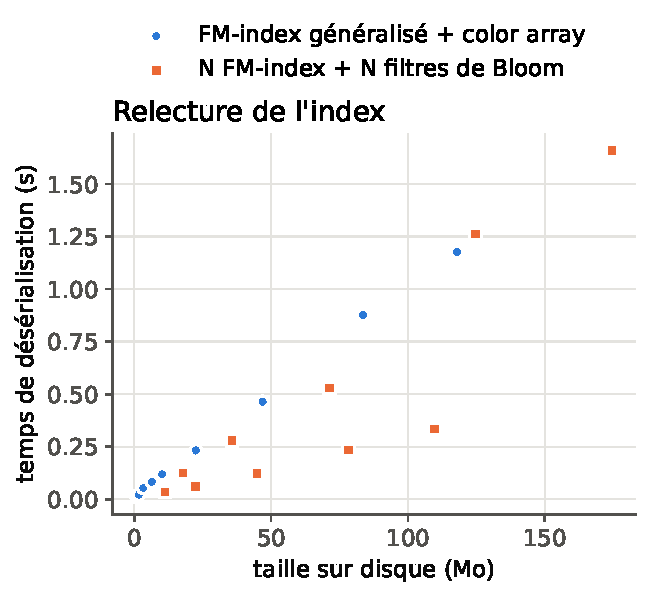
\includegraphics[width=0.5\textwidth]{figures/fig3_deserialisation.pdf}
\caption{\textbf{Temps de désérialisation selon la taille du fichier
sérialisé.} Toutes les configurations E.~coli de l'expérience 1 (10 et
100\,kb, N de 5 à 49). Cité dans le résultat 1.}
\label{fig:deserialisation}
\end{figure}

À taille de fichier égale, l'index \texttt{bf} construit sur des génomes de
10\,kb (les carrés orange les plus bas) se relit 3 à 4 fois plus vite que
\texttt{generalized} (par exemple 110\,Mo en 0,33\,s contre 118\,Mo en
1,17\,s). Ces fichiers sont surtout faits de filtres (des
tableaux de bits relus d'un bloc), alors que relire \texttt{occ} oblige à
recréer un objet Python par entier. Le temps de relecture dépend donc du
nombre d'objets, comme la mémoire vive (résultat 1), plus que du nombre
d'octets.

\end{document}
